%TODO Armar seccion con los graficos 

\subsection{Análisis de corridas - Metodología}

Para poder analizar el comportamiento analizamos los archivos de log para las ejecuciones de los distintos modelos implementados en este trabajo.
El análisis de esta información fue realizado en distintos pasos.

Se tomó el archivo log base que indica qué archivo tiene la información de log para cada modelo.

Con esta información se generó un diccionario con la información de log desglozada según el tipo de evento. Los tipos de mensajes que categorizamos son los descriptos por Wainer. \ref{}

\begin{itemize}
    \item Los mensajes de tipo \textit{*} señalizan la ocurrencia de eventos internos.
    \item Los \textit{X} llevan información de la entrada de eventos externos.
    \item Los \textit{Y} transmiten los eventos de salida.
    \item Los mensajes \textit{done} llevan información de sincronización para futuros eventos, indicando que un modelo ha finalizado su tarea actual.
    \item Los mensajes  \textit{@} o también llamado mensaje de recolección,
        lleva señales para el simulador, indicandole que genere una salida.
    \item Los mensajes \textit{I} marcan la inicialización del modelo.
\end{itemize}

Buscamos analizar distintas variables. Por un lado queremos analizar las componentes estructurales del modelo. Por el otro, entender la evolución en el tiempo de las salidas que arrojan los modelos.

Una estrategia para poder analizar la estructura del modelo es analizar la
cantidad de mensajes enviados por cada modelo. Esto nos habla de la cantidad de
valores de salida emitidos por modelo, de transiciones internas o de eventos
externos que han alterado a nuestro modelo.

Para un modelo sencillo como el de la taza de té generamos gráficos que nos
permiten analizar el comportamiento de la simulación en dos ejes, los eventos
realizados por cada modelo atómico o acoplado.

Para poder generar este, categorizamos cada línea de log para cada modelo y
contamos su frecuencia. Luego, agrupamos estos datos y generamos un Heatmap.
Este gráfico nos permite visualizar las dimensiones \textit{modelo}, \textit{tipo de mensaje } y
\textit{cantidad de ocurrencias} para poder compararlos entre sí.

Dado que el TopLevelCoupled (TLC)  es el orquestador de la simulación, observamos mayor cantidad de eventos de tipo @, Done e Y. La alta frecuencia de eventos Y se explica ya que es el que transporta la información de salida. Dada la diferencia de magnitudes entre los distintos modelos utilizamos una escala logarítmica y una escala lineal para analizar los datos.

Este caso es para la ejecución del modelo de enfriamiento de una taza de té podemos observar que para los modelos FTot, FMinus e Integrador la cantidad de transiciones internas, externas y de salida son iguales. Esto es razonable debido a que estos 3 modelos transicionan inmediatamente.

Para poder analizar el comportamiento de las salidas de cada modelo, utilizamos un gráfico de tipo LetterValue. Este nos indica además de los estadísticos principales (media, percentiles y outliers), la densidad de los valores que se encuentran en un rango de la muestra. Por ejemplo podemos ver que la muestra está no solo centrada en los 70 grados sino que más del 70% de dichos valores se encuentran allí.

Esta información se encuentra en el TLC al igual que cuando se realizó dicha transición.

En esta figura se observa claramente como los modelos de FTot y FMinus no arrojan valores de out. En el caso del Integrador que es el que calcula los valores de temperatura de la taza, es razonable ver que los valores van de 80 grados hasta los 65. Se observa también la alta densidad dentro de los valores cercanos a los 70 grados, momento en el cual debería estabilizarse. Los menores valores pueden tener que ver con el método de integración. Valdría la pena analizar con distintos valores de quantum para entender cuando se generan estos outliers.


\begin{figure}[!h]
	\centering     %%% not \center
	\subfigure[Comparación salida modelo teacup]{\label{fig:teacup_salida_comparada}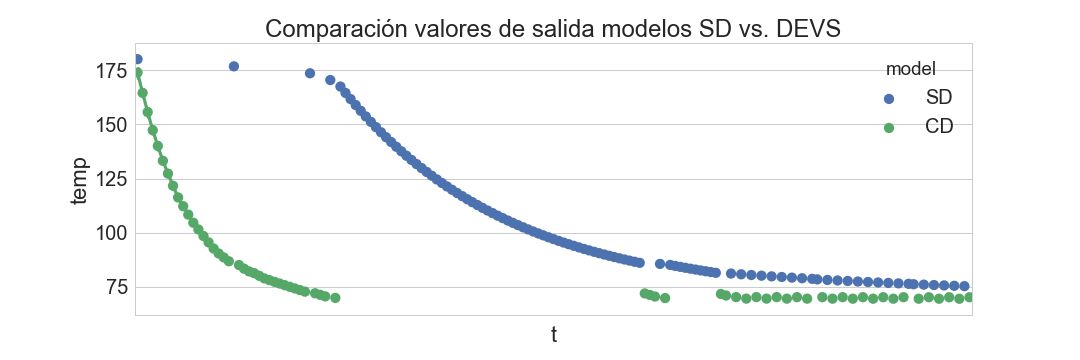
\includegraphics[scale=0.4]{imagenes/tea_comparada_salidas}}


	\subfigure[Cantidad mensajes modelo teacup]{\label{fig:teacup_cant_mensajes}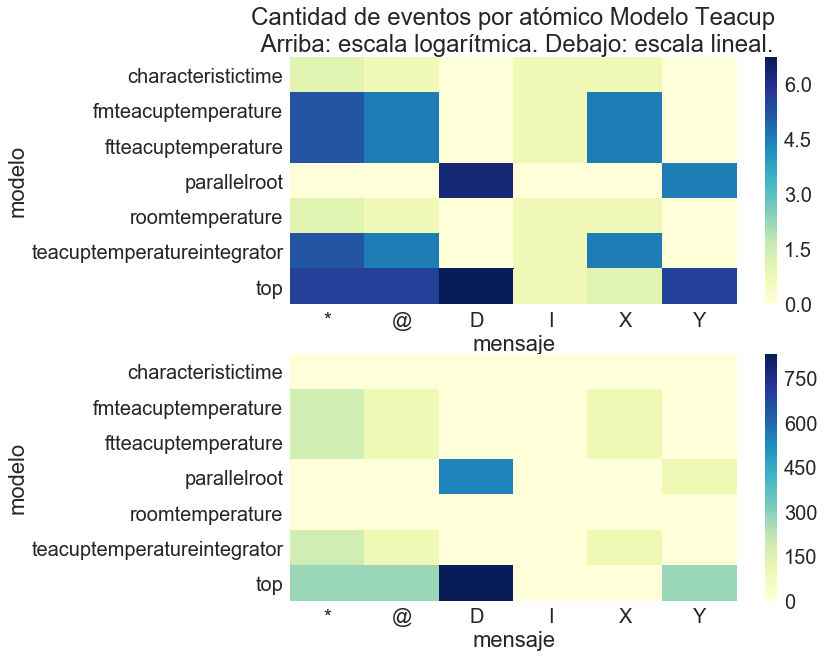
\includegraphics[scale=0.4]{imagenes/tea_cantidad_mensajes}}
	\subfigure[Valores de salida modelo teacup]{\label{fig:teacup_output_letter_plot}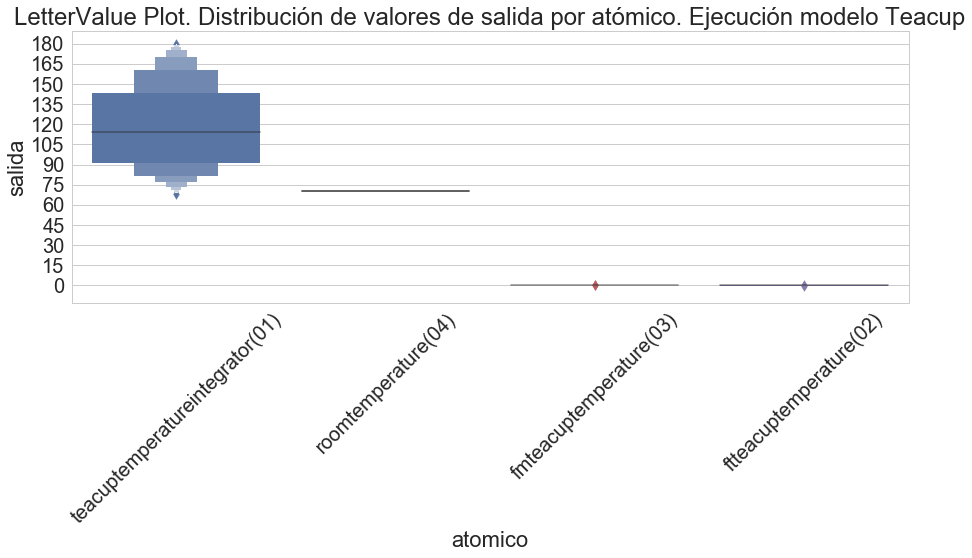
\includegraphics[scale=0.4]{imagenes/tea_output_letter_plot}}
	\caption{Modelo teacup}
\end{figure}

\begin{figure}[!h]
	\centering     %%% not \center
    \subfigure[Comparación salida modelo SIR variable: Infectados]{\label{fig:sir_infect}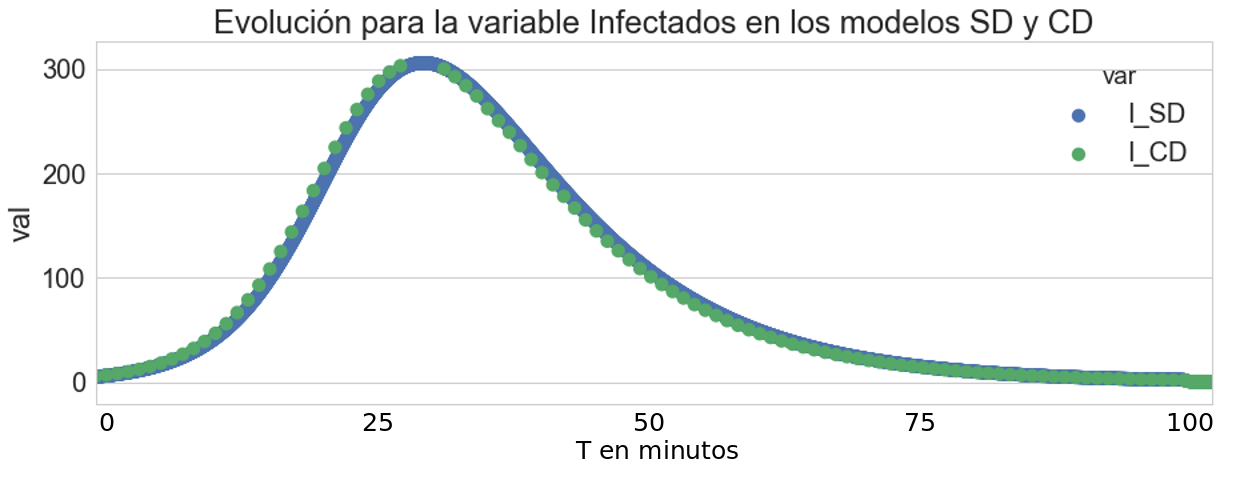
\includegraphics[scale=0.4]{imagenes/sir_comparada_salidas_infectados.png}}
    \subfigure[Comparación salida modelo SIR variable: Recuperandose]{\label{fig:sir_recup}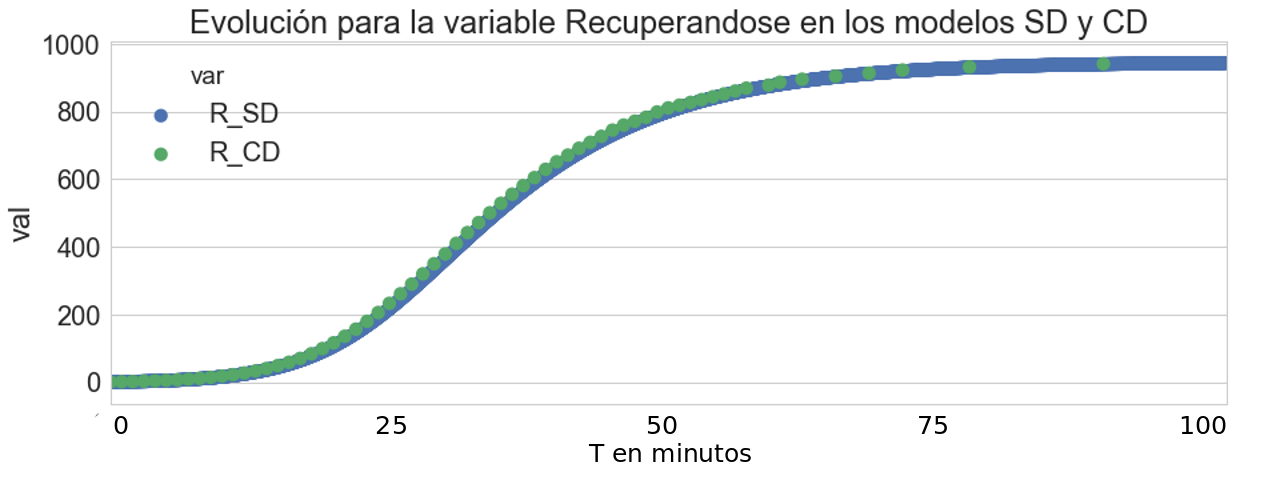
\includegraphics[scale=0.4]{imagenes/sir_comparada_salidas_recuperandose.png}}
    \subfigure[Comparación salida modelo SIR variable: Susceptibles]{\label{fig:sir_sucep}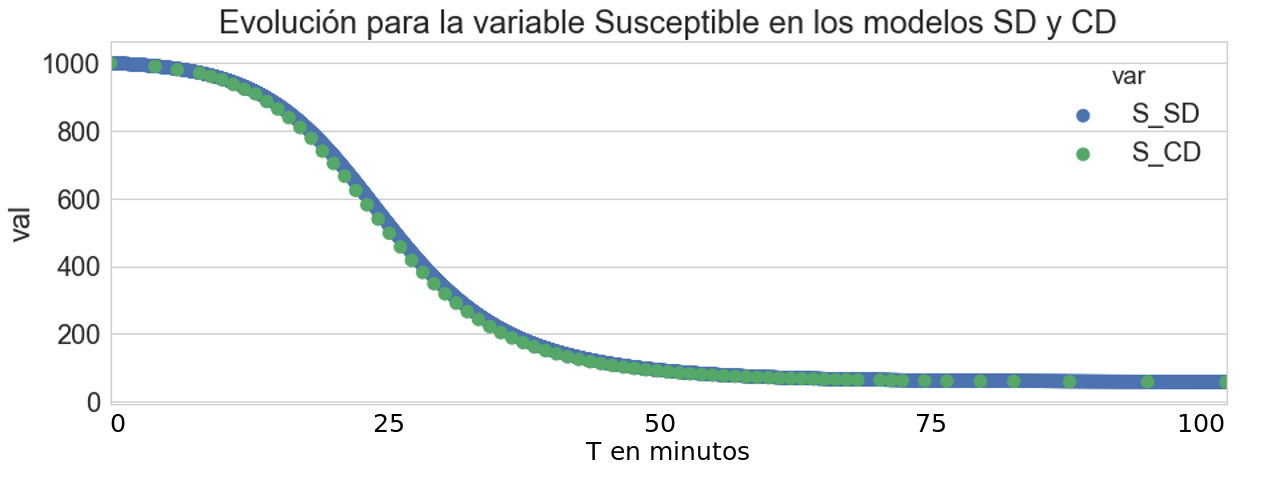
\includegraphics[scale=0.4]{imagenes/sir_comparada_salidas_suseptibles.png}}
	\subfigure[Cantidad mensajes modelo SIR]{\label{fig:teacup_cant_mensajes}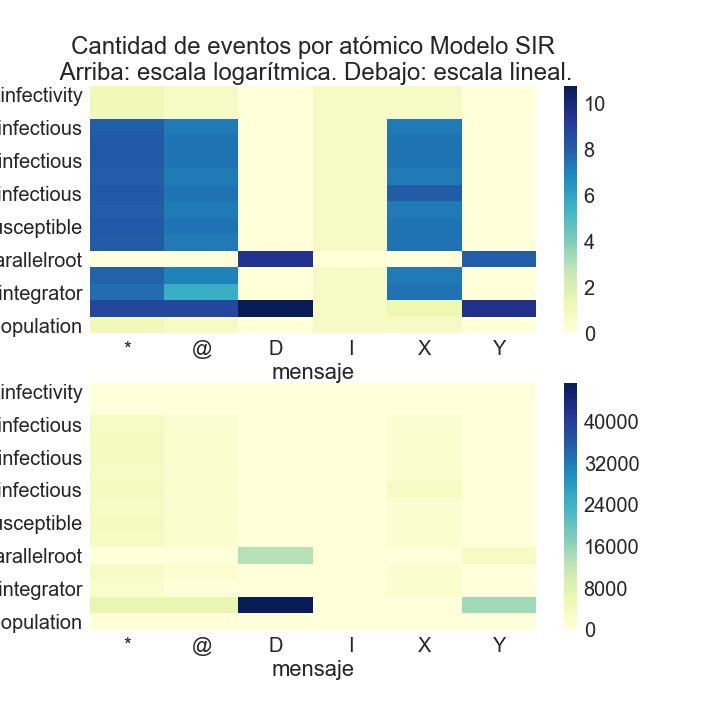
\includegraphics[scale=0.4]{imagenes/sir_cantidad_mensajes}}
	\subfigure[Valores de salida atómicos modelo SIR]{\label{fig:teacup_output_letter_plot}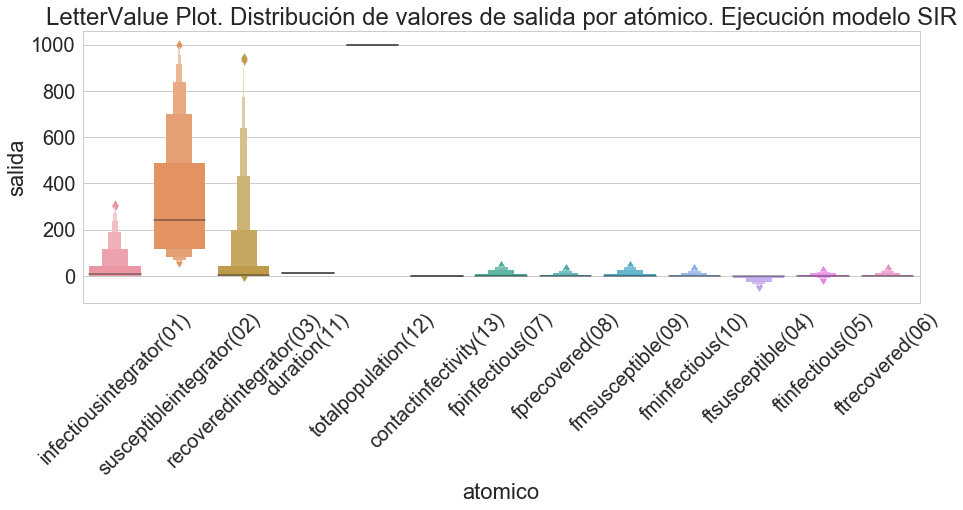
\includegraphics[scale=0.4]{imagenes/sir_output_letter_plot}}
	\caption{Modelo SIR}
\end{figure}
